\section{Mathematical Model}
\label{sec:mathmod}

To model a 3D waveguide \textit{in silico}, the simulation domain must be divided up into regions where specific mathematical relations hold. In this particular system there are three such regions (1) PEC surrounded dielectric, (2) Total Field / Scattered Field (TF/SF) 1-way source, and (3) Mur Absorbing Boundary Condition (Mur ABC). A high level diagram of a PEC bordered rectangular waveguide can be found in Fig. \ref{fig:model}(a) and a $\hat{y}$ sliced model where said relations hold can be found in Fig. \ref{fig:model}(b). These governing relations are then discretized to formulate time-stepping formulas which allow the system to evolve transiently.

\begin{figure}[t!]  
	\centering
	%the command within the [] sets the width of the figure, stability-condition is the jpg name
	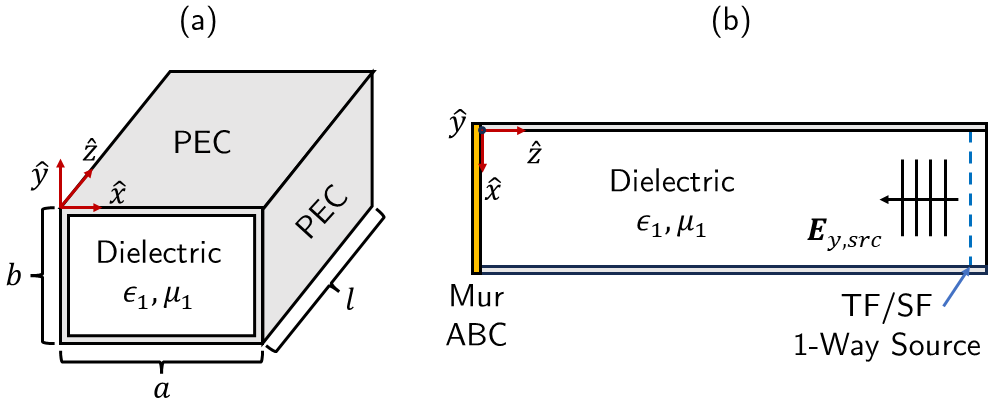
\includegraphics[width=0.9\linewidth]{model} 
	\caption{Diagrams of (a) High-Level PEC Rectangular Waveguide (b) $\hat{y}$-Sliced Model with Labeled Regions}
	\label{fig:model}
\end{figure}

\subsection{PEC Surrounded Dielectric}
\label{subsec:dielectric} 


As seen in Fig. \ref{fig:model}(b) the vast majority of the simulation domain is composed of a PEC enclosed dielectric, the governing equations of which are Amp\`{e}re's and Faraday's Laws respectively. In differential form these, equations take the form 
\begin{align}
    \nabla\times\textbf{H} = \frac{\partial\textbf{D}}{dt} + \textbf{J}
    \label{eq:ampere}
\end{align}
and 
\begin{align}
    \nabla\times\textbf{E}=-\frac{\partial\textbf{B}}{dt} - \textbf{M}
    \label{eq:faraday}
\end{align}
where 
